{\tiny }\section{Úkosy}

Aby bylo jednoduší při zavírání dveře správně natočit, mají zarážky na vnitřní straně velké úkosy, které tak zvětšují na vnitřní straně 
vůli a při zasouvání navedou dveře do správné pozice.


\begin{figure}[htbp]  
    \centering
    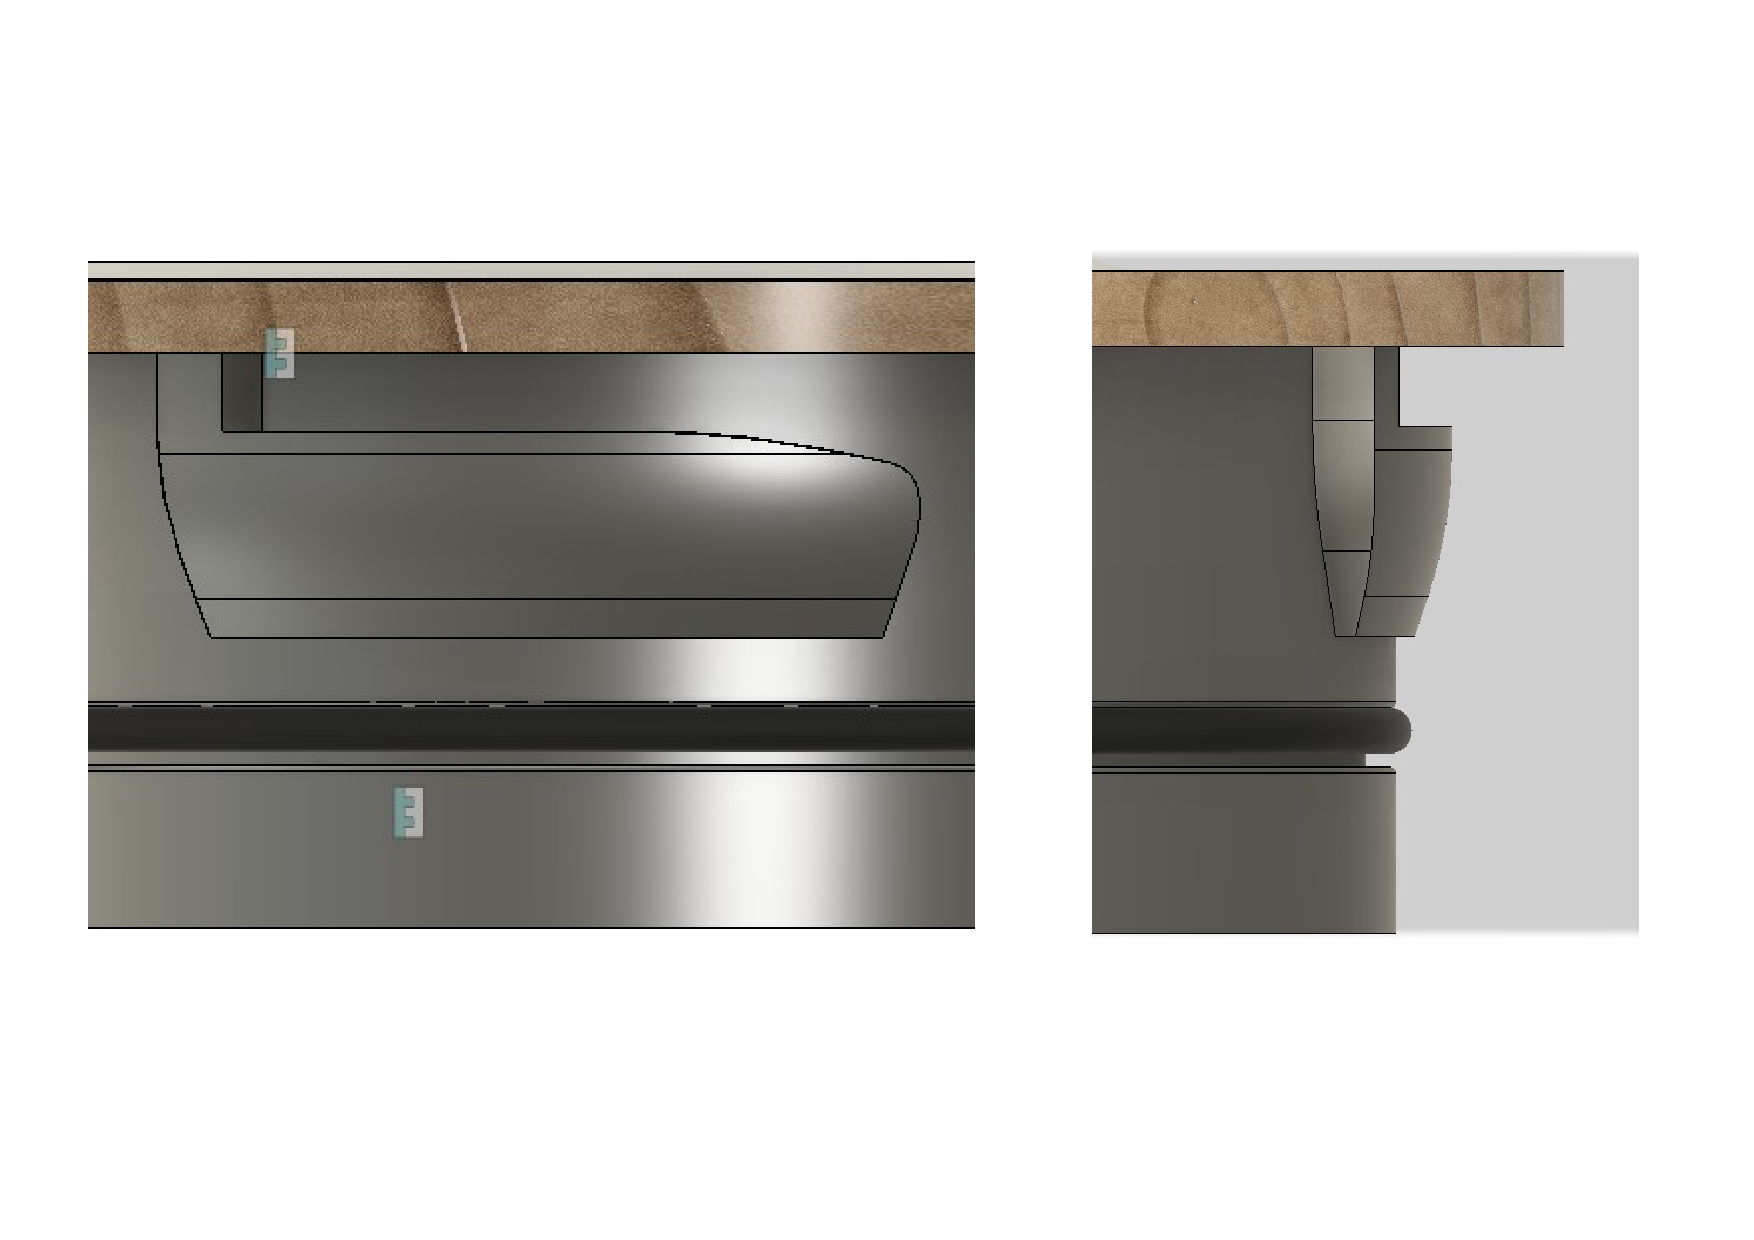
\includegraphics[width=400pt]{kapitoly/obrazky/E4/ukozy/ukladaci_ukosy.pdf}
    \caption{ukládací úkosy}
    \label{fig:E4-ukosy}
\end{figure}

\begin{figure}[htbp]
    \centering
    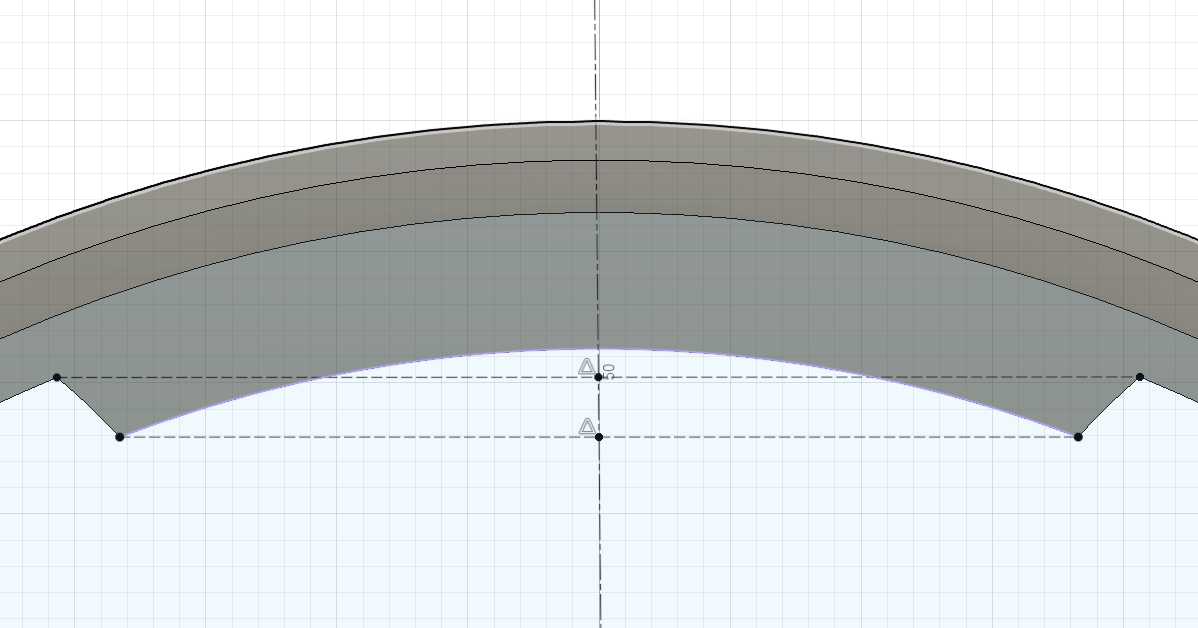
\includegraphics[width=400pt]{kapitoly/obrazky/E4/ukozy/simetrie_zarazek.png}
    \caption{Symetrie zarážky}
    \label{fig:E4-simetrie_zarazky}
\end{figure}
Zarážky na obvodu otvoru mají obě kontaktní plochy stejné. Sice by mohlo být výhodné přizpůsobit tvar strany, kolem které se pohybuje západka, 
pohybu západky. Západka by tak mohla mít vedení v průběhu celého pohybu. Pro symetrii jsem se však rozhodl kvůli možnosti díl s otvorem otočit.
To je zvlášť výhodné při stavbě s dětmi, kvůli zmenšení počtu možných chyb, kterých se děti mohou při stavbě dopustit, a ztráta vedení není tak zásadní.